\chapter{Methods and Implementations}\label{chap:methods}

In this section, we describe our implementations and the specific techniques employed to achieve our results, along with a brief theoretical background when needed.

\section{Trial Wavefunctions}\label{sec:ansatz_closer_view}

\subsection{Standard VMC ansatz}

Our simplest variational ansatz is a parametrised Gaussian and involves no neural network. For a system of $N$ particles and dimension $d$, with a collective position vector flattened as $\mathbf{R} \in \mathbb{R}^{N\cdot d}$, we allow for $N\cdot d$ variational parameters and write
\begin{align}
    \psi_{\mtheta}^{(\text{vmc})}(\mathbf{R}) = \exp\left[-(\mathbf{R} \odot \mathbf{R})^\top\mtheta \right],
    \label{eq:met:single_particle_wf}
\end{align}
where $\odot$ represents element-wise product. When dealing with the log of the wavefunction, we can simply write
\begin{equation*}
    \ln|\psi^{(\text{vmc})}_{\mtheta}(\mathbf{R})| = -\sum_{i=1}^{N d}\theta_i r_i^2.
    \label{eq:met:logsingle_particle_wf}
\end{equation*}

If $\theta_i = 0.5$ for every $i$, this ansatz accurately represents the ground-state wave function of a non-interacting system of bosons at zero Kelvin. It is, however, incapable of satisfying particle-exchange antisymmetry, no matter the choice of parameters, and also fails to satisfy Kato's cusp condition. The antisymmetry requirement can be satisfied by multiplying the ansatz by a Slater determinant, while the cusp condition is addressed via a Jastrow factor ($\mathcal{J}$) or a Padé-Jastrow factor ($\mathcal{P}$), which will be discussed shortly.

The Slater determinant could be any determinant of single-particle orbitals, for example obtained from the Hartree-Fock calculation or the ground state for the non-interacting problem $\Phi_0$, which is how we proceed. We showed in \secref{sec:choice_of_systems} that, for the fermionic problem, the single particle functions $\{\phi_j(\mvec{r}_i)\}$ are a product of a Gaussian envelope and a product of Hermite polynomials for each coordinate $H_{n}(\mvec{r}_i) \equiv H_{n_x}(x_i)H_{n_y}(y_i)\cdots$, where $n$ represents the quantum number. Then, for the VMC ansatz we let the parametrised gaussian be the envelope, and write the VMC Slater ansatz,
\begin{align}
    \ln |\Psi^{(\text{vmc})}_{S}| = \ln|\psi^{(\text{vmc})}_{\mtheta}(\mathbf{R})| + \ln\left|\det\{H_{j}(\mvec{r}_i)\}\right| \label{eq:met:logs}.
\end{align} 

As we discuss in \secref{sec:choice_of_systems}, the block diagonal form of $\{\phi_j(\mvec{r}_i)\}$ further allows us to split it into a product of smaller spin-up and spin-down determinants. Additionally, we will not carry the Slater subscript alone, as every use of the ansatz for fermions will necessarily be accompanied by a determinant of Hermite polynomials.

\subsubsection{Jastrow factor and Padé-Jastrow factor}

The log ansätze, including the Jastrow factor and Padé-Jastrow factor, follow respectively,
\begin{align}
    \ln |\Psi^{(\text{vmc})}_{SJ}| &= \ln |\Psi^{(\text{vmc})}_{S}| + \mathcal{J}_{\mvec{\alpha}}(\mathbf{R}) \label{eq:met:logsj},\\ 
    \ln |\Psi^{(\text{vmc})}_{PSJ}| &= \ln |\Psi^{(\text{vmc})}_{S}| + \mathcal{P}_{\alpha}(\mathbf{R}). \label{eq:met:logpsj}
\end{align}
Both $\mathcal{J}$ and $\mathcal{P}$ introduce inter-particle correlation and depend on the inter-particle distance $r_{ij} = |\mathbf{r}_i - \mathbf{r}_j|$ as
\begin{equation*}
\mathcal{J}_{\mvec{\alpha}}(\mathbf{R}) =  \sum_{i=1}^{N} \sum_{j>i}^{N}  r_{ij}\alpha_{ij},
\end{equation*}
or
\begin{equation*}
\mathcal{P}_{\alpha}(\mathbf{R}) =  \sum_{i=1}^{N} \sum_{j>i}^{N} \frac{a_{ij} r_{ij}}{1 + \alpha r_{ij}}.
\end{equation*}

Note the single variational parameter $\alpha$ in $\mathcal{P}$ instead of a vector. In addition, the factors $a_{ij}$, which depend on the particles $i$ and $j$, are chosen to enforce the ansatz to satisfy Kato's cusp conditions, described in \secref{sec:kato}. For a two and three-dimensional fermionic system, and representing the spin coordinate of particle $i$ as $\sigma_i$, these values were determined by Huang et al. \cite{huang1998spin}, and follow
\begin{equation*}
a_{ij} = \begin{cases} 
\frac{1}{d + 1} & \text{if } \sigma_i =  \sigma_j, \\
\frac{1}{d - 1} & \text{else}.
\end{cases}
\end{equation*}

It should be mentioned that, while we define the Slater-Jastrow and Padé-Slater-Jastrow factors under the VMC ansatz subsection, it can be added to any of the other ansätze presented below. 

\subsection{Restricted Boltzmann Machine Neural quantum states}\label{sec:rbm_nqs}

Given the continuous character of the Monte Carlo sampled values, the restricted Boltzmann machine (RBM) of choice should be Gaussian-Binary. The sampled values for the RBM's visible nodes will indeed correspond to the positions of the particles whose probability distribution is related to the wave function that we aim to obtain. Thus, these will be denoted as $\vec{R}$ rather than $\mvec{v}$ used in \secref{sec:rbm}.

Moreover, the physical quantity we want to sample is related to the marginal probability distribution of the visible units, $p(\Vec{R})$, while the hidden node's values are related to latent variables that do not represent physical quantities of interest. Consequently, we obtain the marginal distribution of interest by integrating $p(\Vec{R}, \mvec{h})$ over the hidden nodes' degrees of freedom,
\begin{align}
    p(\vec{R}) &= \frac{1}{Z}\sum_{\{\mvec{h}\}} e^{-E_{gb}(\vec{R}, \mathbf{h})} \notag \\
                &\propto\sum_{\{\mvec{h}\}} \exp\left\{-\left(\frac{\norm{\mathbf{R} - \mvec{a}}^2}{2\sigma^2}-\mvec{b}^\top\mvec{h} - \frac{\mathbf{R}^\top W\mvec{h}}{\sigma^2}\right)\right\}.  
        \label{eq:marginal}
\end{align}

The proportionality comes from the fact that we do not need the partition function due to the Metropolis sampling. Moreover, we will deal only with hidden units with binary values, so \eqref{eq:marginal} further simplifies, as shown in Appendix \ref{appendix:rbm}. Finally, if we model the probability density of a wavefunction as the marginal distribution probability of the visible units of the RBM, we can write
\begin{align}
   \left| \psi^{(\text{rbm})}_{\mtheta}(\vec{R})\right|^2
                    &=\exp \left\{-\sum_i^{Nd} \frac{(r_i - a_i)^2}{2\sigma^2}\right\}\prod_j^{n_h}\left[ 1 + \exp\left\{b_j + \sum_i^{Nd} \frac{r_i w_{ij}}{\sigma^2}\right\}\right] \label{eq:rbm_trialwf},
\end{align}
where $n_h$ is the number of hidden units, and $\sigma$ is the standard deviation of the Gaussian distribution that the visible units are assumed to follow. In \eqref{eq:rbm_trialwf}, $\mtheta$ serves as a container for all parameters, and for the use of the log wavefunction,
\begin{align}
   \ln \left| \psi^{(\text{rbm})}_{\mtheta}(\vec{R})\right|
                    &=-\frac{1}{2}\sum_i^{Nd} \frac{(r_i - a_i)^2}{2\sigma^2} + \frac{1}{2}\sum_j^{n_h}\left[ 1 + \exp\left\{b_j + \sum_i^{Nd} \frac{x_i w_{ij}}{\sigma^2}\right\}\right] \label{eq:logrbm_trialwf}.
\end{align}

Once again, on its own this trial function does not obey symmetry, antisymmetry, or cusp conditions. Then, the combination of this ansatz with a Slater determinant, or correlation factors is done in analogy to the VMC, equations \ref{eq:met:logs}, \ref{eq:met:logpsj} and \ref{eq:met:logsj},
\begin{align*}
    \ln \Psi^{(\text{rbm})}_{S} &= \ln|\psi^{(\text{rbm})}_{\mtheta}(\mathbf{R})| + \ln\left|\det\{H_{j}(\mvec{r}_i)\}\right|, \\ 
    \ln \Psi^{(\text{rbm})}_{SJ} &= \ln \Psi^{(\text{rbm})}_{S} + \mathcal{J}_{\mvec{\alpha}}(\mathbf{R}) ,\\ 
    \ln \Psi^{(\text{rbm})}_{PSJ} &= \ln \Psi^{(\text{rbm})}_{S} + \mathcal{P}_{\alpha}(\mathbf{R}). 
\end{align*}

Lastly, we should mention that to avoid exploding gradients, $\mvec{a}$, $\mvec{b}$, and $W$ were initialised in a scale inversely proportional to the size of the visible layer, such as $\mathcal{N}_{(0, 0.1)}/\sqrt{N d}$. A similar approach was taken for the feed-forward ansatz, which is our next model.

\subsection{Feed-forward Neural quantum states}

Feed-forward neural networks (FFNs)have also been used to model quantum systems, albeit in a slightly different way than RBMs. This difference comes from the fact that FFNs are not probabilistic or generative models in the same way as RBMs. As there is a clear notion of input and output in this network, we could define the neural network with one output as a function $f: \mathbb{R}^{Nd} \to \mathbb{R}$ and write a simplified ansatz as
\begin{align}
    \psi_{\mtheta}(\vec{R}) = \exp \{f_{\mtheta}(\vec{R})\}\label{eq:ffn_trialwf},
\end{align}
which means that in the log domain, the ansatz is simply the network. Now, if the neural net only admits real parameters, as we defined, the exponential nature of the ansatz could never satisfy antisymmetry under the exchange of particles. There are several methods to guarantee that antisymmetry is satisfied with feed-forward NQSs, with perhaps the most famous implementation being the FermiNet, by David Pfau et. al  \cite{ferminet}. Other successful implementations are also possible and often based on a similar architecture \cite{lin2023explicitly, drissifermion}. The implementation of Pfau et. al, is more intricate than the one we bring here, but a standard Slater-Jastrow ansatz can usually be written
\begin{align}
    \psi_{\mtheta}(\vec{R}) = e^{\mathcal{J}_{\mvec{\alpha}} (\mathbf{R})}\sum_{k} \omega_k \det\{\phi^{k\uparrow}_i(\mvec{r}_j^{\uparrow})\}\det\{\phi^{k\downarrow}_i(\mvec{r}_j^{\downarrow})\},
    \label{eq:sj-ansatz}
\end{align}
where $\omega_k$ are simply weights of the sum. Note that there is not necessarily an explicit separation between a Gaussian envelope and a determinant of polynomials, as the generalised single-particle orbitals $\phi_i^k(\mvec{r}_j)$ can be fully parametrised by the network. 

In first quantisation, the evaluation of several Slater determinants according to \eqref{eq:sj-ansatz} is computationally expensive, but it is also possible to use neural networks in combination with second quantisation formalism \cite{lange2024architectures}. Commonly, the Slater determinants are parametrised by the network which learn transformations that make the single-particle orbitals depend on the configuration, called backflow transformations \cite{holzmann2003backflow}.

We opt to ensure the symmetry of particle exchange using a network architecture based on Deep Sets \cite{zaheer2017deep}. Although this architecture can be used to obtain equivariant layers \cite{jane,drissifermion}, thus ensuring antisymmetry at the architectural level, we do not follow this approach. Instead, we utilised only its permutation invariant implementation and rely on one Slater determinant for antisymmetry.

A permutation-invariant Deep Set consists of writing a neural network as a composition of two functions and a pooling layer in between. We provide here a specific definition of a Deep Set tailored to our applications, rather than a universal definition. For our case, the Deep Set can be written as $\psi_{\mtheta}^{(\text{ds})} =\rho (\Sigma ( \phi))  $ where $\phi: \mathbb{R}^d \to \mathbb{R}^{d_L}$ and $\rho: \mathbb{R}^{d_L} \to \mathbb{R}$. Here, $\Sigma$ represents any pooling operation over $N$, such as the average, for each latent dimension. This can be written $\Sigma :\mathbb{R}^{Nd_L} \to \mathbb{R}^{d_L}$. Moreover, $L_d$ represents a latent dimension, and the architecture can be seen in \figref{fig:deepset}.

\begin{figure}[H]
    \centering
    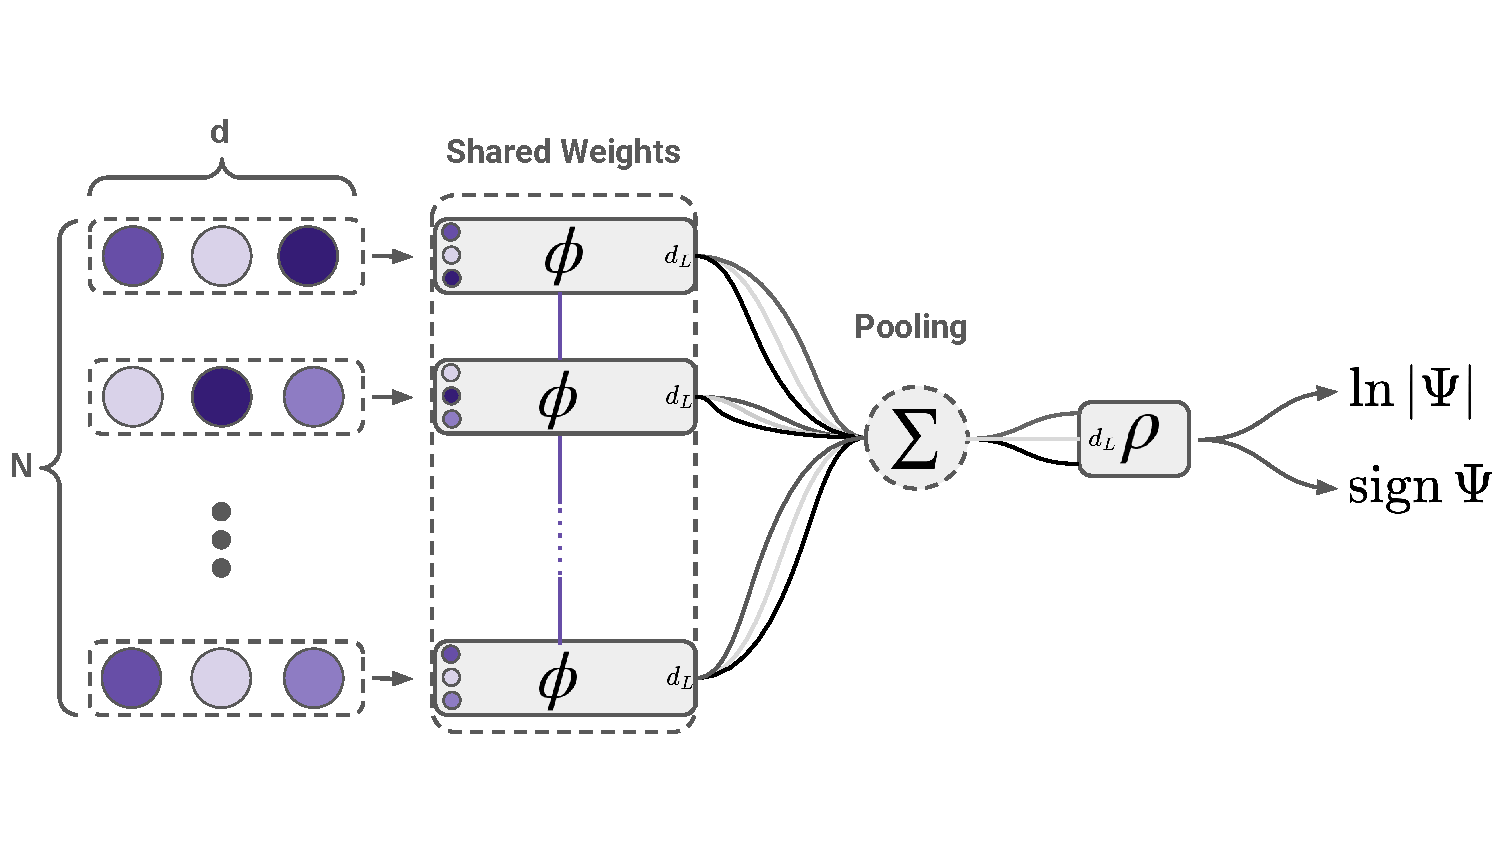
\includegraphics[width=0.9\linewidth]{Chapters/Methods/images/deepset_img.pdf}
    \caption{Representation of a permutational invariant Deep Set architecture. Figure inspired by \cite{jane}.}
    \label{fig:deepset}
\end{figure}

The core idea is that the pooling layer eliminates the specific particle-coordinate association, while the shared weights could theoretically learn inter-particle correlation and encode it to the latent space. This approach scales better than a brute-force symmetrisation in which one sums the outputs for all permuted configurations.

Then, in our code we proceed to use this architecture as the Gaussian envelope, exactly as in the aforementioned methods. Once again, $\psi_{\mtheta}^{(\text{ds})}(\mathbf{R})$ can be multiplied by a Slater-Jastrow or a Padé-Slater-Jastrow factor, yielding
\begin{align*}
    \ln \Psi^{(\text{ds})}_{S} &= \ln|\psi^{(\text{ds})}_{\mtheta}(\mathbf{R})| + \ln\left|\det\{H_{j}(\mvec{r}_i)\}\right|, \\ 
    \ln \Psi^{(\text{ds})}_{SJ} &= \ln \Psi^{(\text{ds})}_{S} + \mathcal{J}_{\mvec{\alpha}}(\mathbf{R}) ,\\ 
    \ln \Psi^{(\text{ds})}_{PSJ} &= \ln \Psi^{(\text{ds})}_{S} + \mathcal{P}_{\alpha}(\mathbf{R}). 
\end{align*}

\subsection{One and Two-Body Densities}

One typical way to analyse many-body correlations is via the one-body density matrix (OBDM),
\begin{align*}
    \rho(\mvec{r}'_1,\mvec{r}_1) = N \int d\mvec{r}_2 \ldots d\mvec{r}_A \Psi^*(\mvec{r}'_1, \mvec{r}_2, \ldots, \mvec{r}_N) \Psi(\mvec{r}_1, \mvec{r}_2, \ldots, \mvec{r}_N),
\end{align*}
which describes the probability amplitude of finding a particle at position $\mvec{r}_1$ while another one is at $\mvec{r}_1'$. For simplicity of visualisation, we have mainly been generating profiles of the diagonal of the OBDM, or the one-body density profile:
\begin{align*}
    n(\mvec{r}_1) = \rho(\mvec{r}_1, \mvec{r}_1) = N \int d\mvec{r}_2 \ldots d\mvec{r}_N \left|\Psi(\mvec{r}_1, \mvec{r}_2, \ldots, \mvec{r}_N)\right|^2 .
\end{align*}

These were obtained by keeping the post-training Monte Carlo sampled positions and displaying on an extra axis the count of how many instances fall under each bin after a discretisation of the space. This will yield a regular histogram for a one-dimensional system or a three-dimensional histogram for a two-dimensional system. The histogram can be normalised so that the density profile integrates to $N$. This is easily done with the NumPy \verb|histogram| function. For the three-dimensional histogram, we further smoothed the plot via a Gaussian filter.

Similarly, the two-body density matrix (TBDM), is a good way to identify higher-order correlation, and is given by
\begin{align*}
    \rho(\mvec{r}'_1,\mvec{r}'_2,\mvec{r}_1, \mvec{r}_2) = N(N-1) \int d\mvec{r}_3 \ldots d\mvec{r}_A \Psi^*(\mvec{r}'_1, \mvec{r}'_2, \ldots, \mvec{r}_N) \Psi(\mvec{r}_1, \mvec{r}_2, \ldots, \mvec{r}_N).
\end{align*}

Its diagonal gives the probability of simultaneously finding two particles at these designated positions $\mvec{r}_1,\mvec{r}_2$:
\begin{align*}
    n^{(2)}(\mvec{r}_1, \mvec{r}_2) = N(N-1) \int d\mvec{r}_3 \ldots d\mvec{r}_N \left|\Psi(\mvec{r}_1, \mvec{r}_2, \ldots, \mvec{r}_N)\right|^2.
\end{align*}

These quantities can be obtained similarly to the OBD profile, where we now bin unique pairs of particle positions. The caveat is that, if using Cartesian coordinates, we would gain a four-dimensional plot, impossible to visualise. However, we can proceed as \cite{Nordhagen2019} and use the radial symmetry of the harmonic trap, reduce the two spatial coordinates to a radial one and disregard the angle. For the sake of visualisation, we then replicate the profile obtained in the four quadrants.


\section{Computational Differentiation}\label{sec:cd}

The methods we employ throughout the thesis have a heavy dependence on the calculations of differentials.

When the derivative of a function is either unknown or we prefer not to calculate it analytically, there are various methods available through computational tools. We will consider computational differentiation to encompass finite difference (FD) methods, symbolic differentiation (SD), and automatic differentiation (AD). When analytical expressions are available, it is advisable to use them rather than rely on computational derivative calculations. This approach will not only be usually quicker but also mitigate the inherent loss of precision that comes with other computational methods.

Each of the above three methods has its advantages and drawbacks. The following is a brief generalisation of some of the important points. One can generally say that symbolic differentiation is inefficient but powerful in that it gives the form of the derivative function to the user. SD is also the best computational method when it comes to sparsity (for example, when a Jacobian matrix is sparse).

Numerical differentiation, together with the related finite difference methods, allows for some control over the precision versus performance trade-off. FD gives a quantification of the precision loss and good generalisability to higher-order differentiation, yet it is dependent on an appropriate and problem-specific choice of step size. The wrong choice leads to large round-off errors in what is called catastrophic cancellation.

For our calculations, except in cases where analytical expressions are used, the method of choice will be AD. AD is very fast and precise and is especially suited to gradient-based optimisations. This is because AD is fast when dealing with partial derivatives with respect to multiple inputs. AD operates by taking advantage of the computational graph that is created when a computer composes simpler arithmetic operations to compute any function. The presence of this composition-like structure in a computer programme enables a straightforward application of the chain rule of partial derivatives to arrive at the final solution. To do that, of course, the programme needs to have access to the function itself, so this method is not applicable in situations where the function is a black box\footnote{Not in the same sense as machine learning black-box but in the sense that the computer has no access to the instructions to be performed for the function output calculation.}.

\subsection{Automatic Differentiation}\label{sec:ad}
Automatic differentiation exists in two variations: forward mode and reverse mode. Understanding this is relevant, especially to explain why our Hessian implementation is actually very efficient. Consider a function $\mathcal{L} : \mathbb{R}^n \to \mathbb{R}^m$, where we write $\mathcal{L}(\mvec{x_0}) = \mvec{y}$. We will denote its Jacobian evaluated at a point $\mvec{x_0}$ in the domain as $\partial_{\mvec{x}} \mathcal{L}(\mvec{x_0}) \in \mathbb{R}^{m \times n}$, or in matrix form:
\begin{align*}
    \partial_{\mvec{x}} \mathcal{L}(\mvec{x}_0) = \begin{pmatrix} \partial_{x_1} y_1 & \partial_{x_2} y_1 & \cdots & \partial_{x_n} y_1 \\ \partial_{x_1} y_2 & \partial_{x_2} y_2 & \cdots & \partial_{x_n} y_2 \\ \vdots & \vdots & \ddots & \vdots \\ \partial_{x_1} y_m & \partial_{x_2} y_m, & \cdots & \partial_{x_n} y_m \end{pmatrix}.
\end{align*}

That function, when calculated in a machine, will be a result of the composition of, for example, $k$ simpler functions $\mathcal{L} = f_k(\cdots f_3(f_2(f_1(\cdot))))$. When applying the chain rule to evaluate the total derivative of $\mathcal{L}$, it is then
\begin{align}
    \partial_{\mvec{x}} \mathcal{L} (\mvec{x}_0) &= \left(\left(\left(\left(\partial_{f_{k-1}} f_k  \partial_{f_{k-2}} f_{k-1} \right)\cdots \partial_{f_{2}} f_{3}\right) \partial_{f_{1}} f_{2}\partial_{\mvec{x}}\right) f_{1}(\mvec{x_0})\right) \label{eq:ad_backward}\\
    &=\left(\partial_{f_{k-1}} f_k \left( \partial_{f_{k-2}} f_{k-1} \cdots \left(\partial_{f_{2}} f_{3} \left(\partial_{f_{1}} f_{2}\partial_{\mvec{x}} f_{1}(\mvec{x_0})\right)\right)\right)\right)\label{eq:ad_forward}
\end{align}

The distinction in computational order between \eqref{eq:ad_backward} and \eqref{eq:ad_forward} is exactly what differentiates forward mode AD from backward mode AD.
When one evaluates the computations from inside-out in terms of the order of the compositions, this is called forward mode. 

The Jacobian itself is a linear transformation and can be seen as a function $\partial f :\mathbb{R}^n \to \mathbb{R}^m$. Furthermore, the chain rule of the Jacobians is, in fact, a set of matrix multiplications. Therefore, while being mathematically equivalent, forward and backward modes do not have the same computational complexity in terms of floating-point operations. Which one is more efficient depends on the problem at hand. For example, if $x\in \mathbb R^{N_0}, f_1\in\mathbb R^{N_1}, \dots, f_k\in\mathbb R^{N_k}$
, backward AD is typically faster if $N_k >N_0$. If $N_k < N_0$, forward AD is favoured \cite{bradbury2018jax}.

From \secref{sec:VMC} we see that VMC will rely on several Laplacian computations, which can be obtained via traces of Hessian matrices. When calculating elements of a Hessian, performing a forward mode over a reverse mode AD or the other way around would both be possible paths. In machine learning applications, however, the function we differentiate often has a wide Jacobian, since a loss function commonly maps to a real number, $\mathcal{L}: \mathbb{R}^n \to \mathbb{R}$. That is why several AD functions are built in reverse mode. Despite that, a Hessian calculation involves the Jacobian of a Jacobian. Since the inner Jacobian will commonly be wide, differentiating it will be better suit for forward mode. Then, forward-over-reverse tends to be more efficient, and this is how we proceed. 

There is of course a case to be made about memory cost. Generally speaking, forward AD is favoured when a neural network is very deep because backward AD requires the storage of more Jacobian matrices.

\section{Just in Time Compilation}\label{sec:jit}
Our current work is done in the Python programming language. This choice is motivated by numerous advantages that Python offers for scientific programming and machine learning, one of which is flexibility, but to the detriment of speed. Although it has had significant improvements in performance in the last years, it still falls short in comparison to purely compiled languages like C++ and Fortran. 

Python has elements of compiled and interpreted languages, and the process of running a Python script can be broadly divided into two parts. First, the source code is compiled by CPython into a lower-level language, bytecode. Bytecode is simply a platform-independent representation of the code but is not yet machine code, and therefore Python is not compiled in the traditional sense. Subsequently, there is an interpretation stage, where the bytecode is fed to a virtual machine. This final stage includes processes such as dynamic type checking and memory management components, along with certain features that offer flexibility but can compromise performance.

Fortunately, with specific tools and some change in code structure, it is possible to compile bytecode to machine code of some functions at runtime - a process called just-in-time (JIT) compilation. JIT compiled functions can be run directly by hardware, helping with interpretation overhead and allowing compiler optimisation and accelerated linear algebra (XLA) techniques to take place. This is particularly valuable in scientific programming, where functions are essentially static, often computationally costly, and must be executed countless times in a simulation.

The design choices that allow for the JIT compilation depend on the framework we use to do so, and there are several Python options. We better explain our JAX \cite{bradbury2018jax} implementation in \secref{sec:jax}, together with several points that require extra care when implementing JIT compilation.


\section{Codebase Overview}

All the code work for this thesis can be found in the Github repository \cite{NQSrepo} and, as it can be used as a Python package, a documentation page is available at \cite{NQSdoc}. The aforementioned pages also contain instructions on how to install the package and run the code. A conceptual representation of the codebase is illustrated in \figref{fig:nqs_overview}. Please note that this diagram does not perfectly map to the repository's modules and is intended to facilitate conceptual understanding. For a detailed view, we refer to the documentation page. We further disclaim that all results were generated on a Mac equipped with an M2 Pro chip and 16 GB of RAM. This machine displayed faster running times than any of the three clusters tested.


\begin{figure}[H]
    \centering
    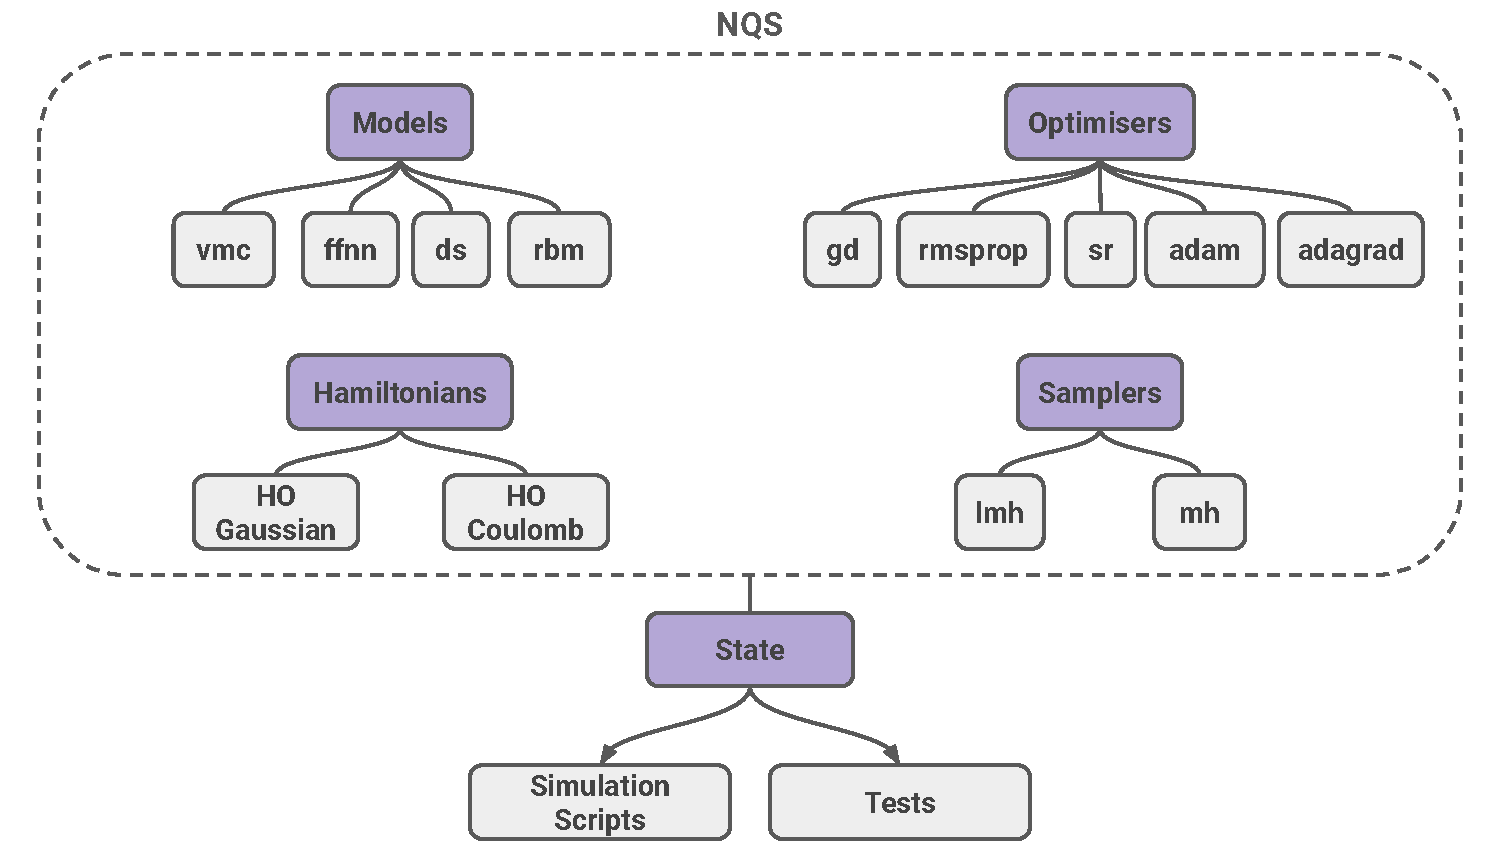
\includegraphics[width=\linewidth]{Chapters/Methods/images/codebase_overview.pdf}
    \caption{Conceptual overview of the NQS codebase, which can be found at \cite{NQSrepo}. See text for explanations.}
    \label{fig:nqs_overview}
\end{figure}

\subsection{Models}

In the project, the term 'models' refers to various choices of ansätze. We have implemented essentially four variants, but only show results for 3 of them. The options are a standard parametrised variational Monte Carlo (VMC), a restricted Boltzmann machine (RBM), a deep-set variant of a feed-forward neural network, and a standard feed-forward neural network for which we do not show results. All of these are implemented to represent the natural logarithm of the absolute value of the wavefunction, for which the sign can always be retrieved with NumPy's function \verb|slogdet|. All models can also be accompanied by a Jastrow factor or a Padé-Jastrow factor.

\subsection{Optimisers}
Following the idea of a modular project, all opitimisers can be used with every model or system, and five options are included: gradient descent (\verb|gd|), adaptative moment estimation (\verb|adam|), root mean square propagation (\verb|rmsprop|), adaptative gradient estimation (\verb|adagrad|) and stochastic reconfiguration (\verb|sr|). Their individual hyperparameters can also be freely modified via the same \verb|set_optimzier| method. 

It should be mentioned that the implementation of stochastic reconfiguration, when used for multilayer networks such as \verb|dsffn| and \verb|ffnn|, approximates the fisher information metric by a block diagonal matrix, as
per \cite{martens2015optimizing}, which we better explain in \secref{sec:kfac}. We chose to continue calling it \verb|sr| to keep consistency, since the VMC and RBM models technically do not use this approximation.

We here display the \verb|set_optimzier| method, and the associated \verb|optimizer_factory|.
\begin{lstlisting}
def set_optimizer(self, optimizer, eta, **kwargs):
    """
    Set the optimization algorithm for parameter updates in the NQS simulation.

    Parameters:
        optimizer (str): The optimizer to use (e.g., 'adam').
        eta (float): The learning rate.
        **kwargs: Additional keyword arguments for the optimizer.

    Raises:
        ValueError: If an unsupported optimizer is specified."""
    self._eta = eta
    common_args = {
        "params": self.wf.params,
        "eta": eta,
    }
    self._optimizer = optimizer_factory(optimizer, **common_args, **kwargs)
\end{lstlisting}

The \verb|optimiser_factory| is responsible for returning the correct class without polluting the main \verb|NQS| class.

\begin{lstlisting}
from nqs.optimizers import Adagrad, Adam, Gd, RmsProp, Sr


def optimizer_factory(opti_type, **kwargs):
    opti_type = opti_type.lower() if isinstance(opti_type, str) else opti_type

    match opti_type:
        case "gd":
            return Gd(**kwargs)
        case "adam":
            return Adam(**kwargs)
        case "rmsprop":
            return RmsProp(**kwargs)
        case "adagrad":
            return Adagrad(**kwargs)
        case "sr":
            return Sr(**kwargs)
        case _:  # noqa
            raise NotImplementedError(
                f"No options for {opti_type}, Only the gd, adam, rmsprop, adagrad and sr supported for now."
            )
\end{lstlisting}


\subsection{Hamiltonians}
The \verb|Hamiltonian| class allows for flexibility in the setup of the physical problem. Any type of particle interaction or external potential can be easily set up. Although it only contains one child class, \verb|HarmonicOscillator|, the type of interaction can be controlled and passed via the \verb|set_hamiltonian| method from the \verb|NQS| class. 

The class is accessed when the method \verb|local_energy| is invoked by the selected sampler, and the measurement is conducted on the wavefunction model object, which is our ansatz.

\subsection{Samplers}

The \verb|Sampler| base class has as child classes \verb|Metropolis| and \verb|MetropolisHastings|, where the latter implements the Langevin Metropolis-Hastings importance sampling described in \secref{sec:langevin_imporance}. 

The base class manages common functionalities, such as setting up the random number generator, logging, and handling the scale parameter for sampling resolution, while the child classes perform the method-specific sampling step. The base class also commands the spawning of parallel but individual Markov chain walkers together with the subsequent collection of statistics from the sampling.

It must be mentioned that our Monte Carlo samplings move all particles at the same time instead of one at a time. Although this is more efficient in terms of random number generation (a large bottleneck in any Monte Carlo calculation), it impedes us from using common tricks to speed up the determinant calculation, such as calculating the determinants via cofactors and updating individual determinant matrix columns. 


\subsection{State}
The State module combines all the pieces of the project in a large class, \verb|NQS|. There, some things can be chosen via their appropriate set methods, such as samplers, models, and optimisers. Although de do not want to include all these methods extensively here, their idea can be illustrated via the set optimser and \verb|set_wf|, the latter being responsible for choosing the ansatz.

\begin{lstlisting}
def set_wf(self, wf_type, nparticles, dim, **kwargs):
    """
    Set and initialize the wave function for the NQS simulation.

    Parameters:
        wf_type (str): The type of wave function to use.
        nparticles (int): The number of particles in the system.
        dim (int): The dimensionality of the system.
        **kwargs: Additional keyword arguments for the wave function initialization.

    Raises:
        ValueError: If an invalid wave function type is provided.
    """
    self.N = nparticles
    self.dim = dim
    self._particle = kwargs.get("particle", "none")
    common_args = {
        "nparticles": self.N,
        "dim": self.dim,
        "rng": self.rng(self._seed) if self.rng else np.random.default_rng(),
        "logger": self.logger,
        "logger_level": "INFO",
        "backend": self._backend,
    }
    specific_args = kwargs
    self.wf = wf_factory(wf_type, **common_args, **specific_args)
    self.nqs_type = wf_type
    self._is_initialized_ = True
\end{lstlisting}

\subsection{Backend}\label{sec:jax}
One of the first things to choose in the NQS class is the back-end, for which the two available options are NumPy \cite{harris2020array} and JAX. In the former, the analytical expressions for the gradients and Laplacians of the ansatz are used, which enables a significant speedup in comparison to JAX automatic differentiation (AD).  However, having the analytical expressions for the gradients is not always straightforward and can limit the great flexibility of deep networks. In our code, using JAX as a back-end is always possible, while NumPy is only allowed for the standard VMC and RBM ansätze, as their analytical expressions can be easily obtained beforehand.

Fortunately, JAX's just-in-time (JIT) compilation speeds up the code considerably, especially when implemented correctly with vectorised maps (vmaps). While we explain AD and JIT in \secref{sec:cd} and \secref{sec:jit}, vmaps are essentially JAX's way of using vectorisation to gain efficiency and readability. 

Unfortunately, extracting JAX's full power requires dealing with some ``sharp bits", in the own words of the project developers. Although we acknowledge that our code may not follow the absolute best practices, it is still relevant to address some of these challenging aspects. For a deeper explanation, we highly recommend the source code and documentation of the framework \cite{bradbury2018jax}.

First, JAX transformations and compilations only work with functions without side effects. This means that ``jitted'' functions, for example, should not modify class attributes or methods if those are not passed as input parameters. This can seem straightforward, but is sometimes difficult to implement when the code design is around object orientation. This requirement of functionally pure code is the reason behind some of the unusual choices in our code, and can be difficult to debug.

Moreover, JAX arrays are immutable and inplace updates need to be substituted from \verb|x[idx] = y| to \verb|x.at[idx].set(y)|. In fact, JAX functions do not deal with NumPy arrays. Fortunately, they are automatically converted to JAX arrays with little to no overhead. 

The minor overhead is the reason we were lax with our array initialisation. For best practices, it would have been preferable to specify the type of array the code is handling from the start, but more often than not, we opted to start with NumPy arrays and let JAX handle the rest. This point is also relevant because we decided not to use JAX's PRNG even when using it as a back-end. 

JAX's RNG is significantly slower than Numpy's defaults, and while there are very good reasons for it, that was not relevant for how we developed our code. We instead leave PRNGs with NumPy, use JAX only for JIT, vmaps and AD, and suffer the overhead from multiple NumPy-to-JAX conversions. In our experience, this was still preferable to using JAX's PRNG.


\subsection{Parameter Class}

We implement the neural nets from scratch, and without pre-built neural network modules. Then, since we want to have a consistent structure for all the possible variational ansatz, we decided to have a specific parameter class.

The \verb|Parameter| class is initialised with a dictionary where the keys are strings representing parameter names, and the values are the parameter data, which can be either NumPy arrays or JAX arrays. This allows for a flexible and extensible structure to hold various types of parameter data.

\begin{lstlisting}
ParameterDataType = Union[np.ndarray, jnp.ndarray]

class Parameter:
    def __init__(self, data: Dict[str, ParameterDataType] = None) -> None:
        self.data = data if data is not None else {}

\end{lstlisting}

The class provides several methods for setting, getting, and manipulating parameter data. The set method is particularly versatile, allowing for setting parameters using different types of input: Replacing the entire parameter data with another Parameter instance, setting multiple parameters using lists of names and values, updating or adding parameters using a dictionary or setting a single parameter using a name and value pair.
\begin{lstlisting}
def set(
    self,
    names_or_parameter: Union[
        str, List[str], "Parameter", Dict[str, ParameterDataType]
    ],
    values: Union[ParameterDataType, List[ParameterDataType]] = None,
) -> None:
    # Method implementation...
\end{lstlisting}

Then, the get method retrieves the value of a parameter specified by name, in the optimisation step. To exemplify, a step of a gradient descent with momentum follows:
\begin{lstlisting}
def step(self, params, grad_params_E):
    for key, grad in grad_params_E.items():
        self.v[key] = self.gamma * self.v[key] + grad
        params.set([key], [params.get(key) - self.eta * self.v[key]])
\end{lstlisting}

One of the key aspects of this class is its integration with JAX's tree utilities, which is essential for enabling JAX's automatic differentiation and other optimisations. The \verb|tree_flatten| and \verb|tree_unflatten| methods are implemented to allow the Parameter class to be used with JAX's \verb|jit|, \verb|grad|, and other transformations. The \verb|tree_flatten| method breaks down the Parameter object into a list of its values (leaves) and a list of keys (auxiliary data). This decomposition is necessary for JAX to understand and manipulate the data structure during computation.

Finally, the \verb|Parameter| class is registered with JAX using the \verb|register_pytree_node| function. This registration tells JAX how to handle instances of the \verb|Parameter| class during its computations.

\subsection{The Wavefunction Base Class}

The \verb|Wavefunction| base class is inherited by any choice of ansatz or model, allowing for modularity. Its design ensures that common functionalities are handled in one place while allowing specific behaviours to be defined in child classes. It, for example, controls, via abstract class methods, the setput of the Slater determinants and the Jastrow factors regardless of the trial function. This is because specific methods are called in the constructor of its child classes.

Very importantly, too, this class enables the setup of the appropriate backend (NumPy or JAX), and the just-in-time compilation for the appropriate functions. 

\subsection{Simulation Scripts}

The simulation scripts in this repository manage the entire simulation process. They outline the steps for initialising models, configuring Hamiltonians, choosing and executing samplers, carrying out optimisation, and also gathering the results. These scripts are created to be modular and flexible, enabling easy modification of parameters and settings. This means that almost all options can be arbitrarily combined. For example: any model can take any particle type and use any optimiser, any sampler, and any Hamiltonian. We refer to Appendix \ref{sec:minimal_nqs} for a minimal display of one of these simulation scripts.




\section{General Training Strategies}

In this section, we present a variety of implementation techniques that were crucial to achieving satisfactory results.

\subsection{Pretraining and regularised potential}\label{sec:pretrain}

Throughout our implementations, we make use of the method of transfer learning. Transfer learning consists in loading the weights of a model trained in a similar problem to accelerate the convergence when using the network in other scenarios. More specifically, this was a crucial step in obtaining reasonable convergence when minimising the energy of interactive systems with multilayer network ansatz. In dimensions larger than 1, we did not manage to get stable sampling without it, giving positions in a clearly unbounded way.

First, we pretrain the network to a supervised regression task, in which we regress the log-probability $\ln(|\psi|^2)$ of the ansatz to the log of a multivariate Gaussian with identity covariance matrix of dimension $(N\times d) \times (N\times d)$, where $N$ is the number of particles, and $d$ the number of dimensions. This is to ensure that the network at least starts with a function with a vanishing profile for large coordinate values.

The second stage involves either pretraining the network to the non-interactive related system, or training in a regularised potential that converges to the true interaction potential towards the end of the training process.

Both these second-stages consist in training the model within the standard VMC - reinforcement learning framework, but the details vary based on the system. If the particle interaction does not exhibit singularities, we pretrain the ansatz to converge to the non-interacting system. Else, we regularise the potential, adopting a method inspired by \cite{jane}.
While this regularisation and pretraining are different techniques, the regularisation process essentially introduces the interaction slowly and in a specific way that hopefully helps the network learn Kato's cusp condition without the need to impose a fixed Jastrow factor. This regularisation consists of using a potential
\begin{align*}
    \frac{1}{r_{ij}} \to \frac{\tanh(r_{ij}/r_0)}{r_{ij}}
\end{align*}
where $r_0$ is a hyperparameter. The numerator in this regularisation can be any function of $r_{ij}$ such that $f(r_{ij})$ approaches 1 as $r_{ij}$ approaches 0. 
More specifically, in our implementations we add a decay rate $\tau$ to $r_0$,
\begin{equation}
    \tau = \left(\frac{1}{3 r_0}\right)^{2/T},
\end{equation}
such that, at half of the training process, $\tanh(r_{ij}/r_0) \approx 0.97$. Here, $T$ is the total number of training epochs, and at each iteration, we change $r_0(t) = r_0(0)\cdot\tau^t$, where $t$ is the current epoch. When sampling the observables from the final ansatz after training is done, we simply turn off this regularisation so that the ansatz is kept fixed.

\subsection{Sampler Tuning}

The quality of a Monte Carlo sampling is heavily influenced by the width of the distribution that is sampled from. In our implementations, this width is simply called the scale of the Monte Carlo method. In order to obtain an efficient sampling process, one usually aims at finding a sample width that yields approximately 50\% of accepted moves. To achieve that, we created a \verb|tune_scale| method based on the PyMC library \cite{pymc2023}, but with some minor modifications.

In the PyMC implementation, the method adjusts the proposal scale for a sampler based on the acceptance rate, aiming for an optimal range between 20-50\%. Our approach differs by targeting an acceptance rate of 50-70\%. Furthermore, our method activates only when the acceptance rate falls outside the 30-70\% range, to avoid unnecessary tuning. These target values were determined experimentally, without a rigorous experimentation process.

The tuning process operates via a lookup table that adjusts the proposal scale according to predefined acceptance rate thresholds. If the acceptance rate is extremely low (<0.001) or extremely high (>0.99), we reinitialize the sampling positions and the weights of the ansatz without stopping the training process. This decision comes from observing that such acceptance rates indicate that the walkers have wondered into regions of impossible convergence, often due to an ill-defined ansatz.

When tuning the sampler, some considerations must be made. One of these is the batch size used to evaluate the acceptance rate. This batch size can be larger than the training batch size for higher precision in the tuning phase or smaller for faster execution. Another key consideration is whether to exit the tuning process if the optimal acceptance rate range is not met.

To address this last point, we devised two methods for the tuning process. The standard method allows setting a maximum number of iterations for the tuning process. If the acceptance rate does not fall within the optimal range within these iterations, the process stops. In contrast, the infinite method continues the tuning indefinitely until the acceptance rate falls within the desired range.

\subsection{Clipping gradients and energy values}
Lastly if should be mentioned that we implemented clipping strategies in two instances to obtain numerical stability. First, following an approach similar to \cite{ferminet}, the local energy values during network training are clipped according to the $\ell_1$ norm. Specifically, the average local energy $\langle E_L\rangle $ is kept only if it falls within the range $\langle E_L\rangle \pm 5 \times \langle | E_i - \langle E_L\rangle |\rangle$.

Another strategy that was implemented by us but not thoroughly examined was gradient clipping. Gradient clipping consits in rescalling the gradient vectors to have a smaller norm, while still pointing to the same direction in space. This has been shown to help with training convergence in regions where the loss landscape has abrupt changes. Essentlially it consits in defining a threshold $\rho$ and redefining $ \nabla \mathcal{L}$ if $\norm{\nabla \mathcal{L}} > \rho $ to 
\begin{equation}
    \nabla \mathcal{L} \leftarrow \frac{\rho \nabla \mathcal{L} }{\norm{\nabla \mathcal{L}}}.
\end{equation}


\subsection{Parallelisation}\label{sec:parallel}

Good statistics of the quantities obtained via Monte Carlo simulations are heavily dependent on how much data we are able to generate. Assuming that the simulated data represent independent and identically distributed sub-samples of the quantity we are trying to infer, the law of large numbers ensures that having a larger number of points will result in a better reconstruction of the true probability distribution.

One reliable way to obtain more data for Monte Carlo simulations in a similar amount of time is to collect samples from parallel random walkers. This means that simulations are run in parallel and that their individual sampled values can be combined to compose a larger collection of the final data. One important assumption for this parallelisation process is that random walkers are unaware of each other, so the samples do not exhibit undesired correlations, compromising the statistical significance of the computations. This requirement can be satisfied by passing unique random seeds for the different threads of the parallel programme. 

In particular, for our Python parallel sampler implementation, we used the Joblib \cite{joblib} library. The motivation for using Joblib instead of Python's native multiprocessing module is that the latter displayed problematic behaviour when sharing JAX objects among processes. Joblib's \verb|parallel| function achieves embarrassingly simple parallelisation by starting separate Python workers that execute tasks on different CPUs.


\section{Quantifying uncertainties}\label{sec:blocking}
There are multiple ways to analyse the statistical uncertainty of the collected data. Most standard methods rely on resampling techniques, which artificially generate more data by creating varied samples from the limited data set. For example, by shuffling data and resampling it, one can achieve a finer statistical estimation of the measured quantities due to the larger amount of data, hopefully without biasing it too much.

Conventional implementations include bootstrapping and cross-validation, better explained in \cite{hastie2009elements}. VMC calculations deal with a very large amount of data, making these approaches computationally costly. More importantly, perhaps, these methods also do not explicitly take into account the correlation between data points, an important feature when analysing how the random walks evolve in configuration space. Of course, at a stationary limit, sample averages should be time independent, but in practice we do not have this guarantee. Therefore, specifically for VMC calculations, the blocking method is often used. 
 
Quantities measured in a Monte Carlo sampling are the results of a set of sequential experiments, $\{\alpha\}$. The sampled values, such as the mean ($\mu_\alpha$) and variance ($\sigma_\alpha^2$) of these experiments, can therefore be studied as a time series. Here, these quantities are given by
\begin{equation}
    \mu_{\alpha}=\frac{1}{N}\sum_{k=i}^N x_{\alpha, k}, \qquad \sigma^2_\alpha=\frac{1}{N}\sum_{k=1}^N(x_{\alpha, k} -\mu_\alpha)^2.
\end{equation}

The entire data set can be partitioned into $m$ experiments blocks, with its $m$-th block having an average $\mu_{m}$ with a sample mean variance $\sigma^2_m$; both can be written as
\begin{align}
    \mu_{m}=\frac{1}{mN}\sum_{\alpha, k} x_{\alpha, k}, \qquad  
    \sigma^2_m= \frac{\sigma^2}{N}[1 + 2\sum_{d=1}^{N-1}k_d],
    \label{eq:blocking_std}
\end{align}
where $\sigma^2$ is the variance of all the data points,
\begin{equation*}
    \sigma^2 =\frac{1}{mN}\sum_{\alpha k}(x_{\alpha, k} -\mu_m)^2,
\end{equation*}
and $k_d$ is the autocorrelation function \cite{park2018fundamentals} between experiments separated by a distance of $d$ in the time series. The blocking algorithm consists of rearranging the total data set into blocks and analysing how $\sigma_m^2$ changes with different block sizes. When the number of blocks increases, this variance of the average of the blocks reaches a plateau that gives information about the correlation of the experiments. The aim is to find a distance $d = |k-l|$ between sequential experiments $x_{\alpha, k}$ and $x_{\alpha, l}$ such that experiments in the time series separated by a distance $d' > d$ can be considered uncorrelated. The standard deviation provided by the blocking algorithm will then be the asymptotic value that stabilises for this distance $d$. This is clear from \eqref{eq:blocking_std}, as $\sigma^2_m \to \sigma^2/N$ if $k_d$ tends to 0.

In our implementation of the blocking algorithm for the estimation of the standard deviation of the energy, we used the systematised scheme of \cite{jonssonStandardErrorEstimation2018}. This method automates the ordinary visual analysis of the time auto-correlation function devised by \cite{flyvbjergErrorEstimatesAverages1989}. 

\subsection{Combining errors}
We have discussed the use of parallelisation techniques in Python to produce more samples in roughly the same time frame via parallel computing and multiple CPUs. Here, we give a more detailed explanation of how we aggregated the errors from each independent experiment.

The empirical expected values and their variances are also random variables, and to appropriately combine mean values and standard errors, we used a meta-analysis study. More specifically, we use inverse variance weighting (IVW) \cite{borenstein2021introduction} to aggregate the values of random variables so that their average is weighted by the inverse of their variance.

After running $n$ independent walkers, each will give us an empirical expectation value of the energy $E_n$, with its associated blocking error $\text{SE}(E_n)$. Then, we use IVW to combine these values into a single overall estimate of energy $\bar{E}$ and its associated error $\text{SE}(\bar{E})$ as follows:
\begin{equation*}
\bar{E} = \frac{\sum_{i=1}^n w_i E_i}{\sum_{i=1}^n w_i},
\end{equation*}
with the weights determined by the inverse variance of each estimate $w_i = \text{SE}(E_i)^{-2}$. Then, the standard error of the mean estimate is given by
\begin{equation*}
\text{SE}(\bar{E}) = \sqrt{\frac{1}{\sum_{i=1}^n w_i}}.
\end{equation*}

\section{Kronecker-factored Approximate Curvature}\label{sec:kfac}

In practical applications, particularly with the emergence of deeper and broader networks in deep learning, calculating the complete Fisher information matrix or its quantum counterpart, the Fubini study metric, becomes impractical. Not only is it computationally demanding to invert the matrix $F_{ij}$ as required by the update rule, but storing the matrix elements also becomes memory intensive. Indeed, in a naive approach, one must recompute and store its values for each training iteration. 

If we consider a rectangular neural network structure, in which all $L$ layers have the same height $H$, and further assuming that there are no bias vectors, the FIM should be a matrix of size $(L \times H^2) \times (L \times H^2)$. Kronecker-factored approximate curvature (KFAC), devised by Martens and Grosse in 2015 \cite{martens2015optimizing} is a technique that aims to simplify this structure in two ways. In this brief explanation, we do not provide a derivation of the expressions, and for a detailed proof, we refer to the original publication.

Using the notation of \cite{drissi2024second}, we start by approximating the FIM by a block-diagonal $\breve{F}$,
\begin{align}
    \breve{F}(\mvec{\theta})_{W_{ij}^{(l)}{W^{(l')}_{i'j'}}} \equiv \delta_{ll'}\, F(\mvec{\theta})_{W_{ij}^{(l)}{W^{(l')}_{i'j'}}},
\end{align}
where $W_{ij}^{(l)}$ represents a weight matrix of given layer $l$, and $\delta_{ll'}$ a Kronecker delta. This means that we assume parameters from different layers of the network to be independent in terms of the curvature of the parameter space. This turns the $(L \times H^2) \times (L \times H^2)$ matrix into $L^2  H^2$ blocks of $(H\times H)$ matrices that can be inverted independently.

The second simplification of the KFAC method consists of writing the blocks of the approximated $\breve{F}$ as Kroneker products of statistical averages of the forward activations $\Vec{a}^{(i)}$ and backward sensitivities $\delta^{(i)}$ of the FFN, discussed in \secref{sec:training a FFN}. Then, it can be shown that 
\begin{align}
    \breve{F}(\mvec{\theta})^{(l)} \approx \mathbb{E}_{p_\theta}\left[\Vec{a}^{(l)}\Vec{a}^{(l-1)^\top}\right]\otimes\mathbb{E}_{p_\theta}\left[\delta^{(l)}\delta^{(l-1)^\top}\right].
\end{align}
However, throughout this work, we do not implement this last simplification.

\subsection{Trust regions and Tikhonov regularisation}

When solving second-order optimisation problems practically, the constrained minimisation problems of \eqref{eq:steepst_argmin} and \eqref{eq:newtons_minimisation}, discussed in \secref{subsec:Learning as opt} are often treated as analogous unconstrained problems with associated trust regions and damping parameters, in what is called the Tikhonov regularisation method. More specifically, consider the second-order approximation model
\begin{equation*}
M(\delta) = E(\boldsymbol{\theta}_0) + \nabla E(\boldsymbol{\theta}_0)^\top \delta + \frac{1}{2} \delta^\top G \delta,
\end{equation*}
where 
$\delta = \mvec{\theta} - \mvec{\theta}_0$ , and 
$G$ is a matrix describing the geometry of the trust region. For example, in Newton's method, it is the Hessian of the objective function, and in the natural gradient method, it is the Fisher information matrix. Following Tikhonov regularisation, the correct update rule is given by the unconstrained minimisation,
\begin{align*}
    \mvec{\theta}_{t+1}- \mvec{\theta}_t = \arg \min_{\delta\in R_t} \left(M_t + \frac{\lambda_t}{2} \delta^\top G(\theta_t)\delta\right),
\end{align*}
where, $\lambda$ is the damping term and $R_t = \{\delta : \norm{\delta} \le r_t\}$, for some radius $r_t$, is a trust region for which the second-order approximation is valid. Adding this damping term has the effect of using a regularised version of the FIM, equivalent to $F - \lambda I$. This is important to stabilise the pseudo-inverse calculation of $F$ via singular value decomposition. In our work, we have used a diagonal shift of around $\lambda = 10^{-4}$.

In reality, choosing the correct radius of the trust region at every step is impractical, and learning rate decay schedules have been suggested to ameliorate this difficulty \cite{glasser2018neural}. For our implementations, we proceeded by choosing the learning rate
\begin{equation*}
     \alpha_t = \min\left(\alpha_0, \sqrt{\frac{\alpha_1}{\delta_\theta^\top G \delta_\theta}} \right)= \min\left(\alpha_0, \sqrt{\frac{\alpha_1}{(F^{-1} \nabla E(\theta))^\top \nabla E(\theta)}} \right),
\end{equation*}
with $\alpha_0$ and $\alpha_1$ hyperparameters that require tuning. This is an idea suggested in \cite{sheng}, which requires that the scheduler choice could depend on the curvature of the trust region. This choice ensures that the learning rate is smaller when the curvature of the parameters under the metric defined by $G$ is large. In addition to that, we also added a momentum term of $\gamma = 0.9$ in our implementations. Then, the update rule when implementing specifically our version of SR can be written 
\begin{align*}
    \mvec{v}_t &= \gamma \mvec{v}_{t-1}  + \breve{F}^{-1}\nabla E(\theta), \\
    \mvec{\theta}_{t+1} &= \mvec{\theta}_{t} - \alpha_t\mvec{v}_t,
\end{align*}
where we denote $\breve{F}$ as the block-diagonal approximation of the FIM.

\section{Hyperparameter Search}\label{met:param_search}

Optimising hyperparameters is a crucial part of training machine learning models, as it can greatly influence the quality of the model. Performing extensive brute-force searches over the hyperparameter space is a task that is intractable on its own, as the number of possible configurations scales exponentially. To find the best configuration for a certain model, several techniques can be employed, the simplest being random selection over the parameter space. 

Several of our initial investigations to find a good choice of model and parameters begin with a trial-and-error process, as this carries a lower overhead in initial iterative phases of a project. However, for more detailed and subsequent investigations, when the aim is to find the best model, we utilised the Weights \& Biases (Wandb) software \cite{wandb}. This is a well-known tool for experiment tracking and hyperparameter tuning, supporting the automation of hyperparameter searches through Bayesian optimisation and randomised search. Parameter searches using Wandb will hereafter be called sweeps, following the software convention.

We opted to proceed in a slightly different manner depending on the system being investigated. For the fully polarised one-dimensional fermionic system, the runs are executed reasonably quickly, as we deal with a one-dimensional problem and we only gather results for up to 6 fermions. In this scenario, when generating sweeps over the entire set of parameters, we select several hyperparameters such as batch size, neural network architecture, learning rate, whether to use a pretraining stage, the type of optimiser to use, whether to use regularisation, and others.

In one-dimensional runs, we conducted three major sweeps, one for each ansatz type: Deep Set feed-forward net (DSFFN), standard variational Monte Carlo (VMC), and restricted Boltzmann machines (RBM). Here, the sweeps include uniform random selection over the number of particles and interaction strength. This affects the energy to which we are converging, but the software enables filtering runs afterward, extracting averages for specific combinations of number of particles and interaction strength. The large number of sweeps ensures a fair representation of the hyperparameters in a uniform search. For instance, we have roughly the same number of runs using stochastic reconfiguration and Adam as optimisers for two, four, and six particles alike.

When dealing with two-dimensional quantum dots, the additional dimension and the increased number of particles make the computations more expensive, so we adopted a different approach. Here, we explicitly separate the investigation into exploration and exploitation phases. The exploration phase involves performing sweeps over hyperparameters for several short runs (with a small number of epochs and batch sizes for the Monte Carlo averages). To do this efficiently, we used a random Bayesian optimisation search instead of a uniform random search. 

Bayesian optimisation is an efficient strategy for hyperparameter tuning, especially when the evaluation of configurations is expensive, or there are simply too many configurations to try \cite{dewancker2016bayesian}, which is often the case with deep learning models. Bayesian optimisation works by building a probabilistic model (typically a Gaussian process) of the objective function and using information of previous parameter choices to select the most promising hyperparameters to evaluate next.

After these short sweeps, we select the hyperparameters from which we want to collect statistics. This stage requires a modification of how we separate the sweeps. This is because, in Bayesian optimisation, we must specify the metric to be minimised beforehand. If we include configurations with varying numbers of particles in a single Bayesian sweep and use the expected energy value as the objective function, systems with fewer particles will be favored because they have lower energy. One option to circumvent this could be to guide the Bayesian search to minimise the variance of the energy instead. Nevertheless, even though variance optimisation has an absolute target (0 at the ground state), larger systems are intrinsically harder to train because of multiparticle interactions and correlations. Consequently, simpler systems would be selected more frequently.

For two-dimensional systems, we opted to conduct separate Bayesian sweeps for each number of particles. Furthermore, we only perform sweeps for a harmonic trap frequency of $\omega = 1$, in the hope that the best model will be able to generalise well for different frequencies in subsequent simulations.


